\documentclass[runningheads]{llncs}
\usepackage[T1]{fontenc}
\usepackage{graphicx}
% Used for displaying a sample figure. If possible, figure files should
% be included in EPS format.
%
% If you use the hyperref package, please uncomment the following two lines
% to display URLs in blue roman font according to Springer's eBook style:
%\usepackage{color}
%\renewcommand\UrlFont{\color{blue}\rmfamily}
%
\begin{document}
% Just after the begin
%\begin{document}
\begin{titlepage}
    \centering
    {\bfseries\LARGE International University of Ecuador \
        Faculty of Technical Sciences  \par}
    \vspace{1cm}
    {\scshape\Large School of Mecatronics engineering \par}
    \vspace{3cm}
    {\scshape\Huge Industrial Automatization \par}
    \vspace{3cm}
    {\itshape\Large Lab's Preparatory No 2:  \par}
    \vfill
    {\Large Authors: \par}
    {\Large Sebastian Osorio \\ Pablo Guacho \par}
    \vfill
    {\Large Sep 20222 - Jan 2023 \par}
\end{titlepage}
\newpage
\title{Lab's preparatory No. 2\thanks{UIDE.}}
%
%\titlerunning{Abbreviated paper title}
\author{Sebastian Osorio\inst{1}\orcidID{0000-0003-0106-5482} \and Pablo Guacho\inst{1}\orcidID{0000-0003-0106-5482}}

\authorrunning{S. Osorio, P. Guacho.}

\institute{International University of Ecuador, Quito Av. Jorge Fernández and Av. Simón Bolívar 170201, Ecuador
    \email{uide@uide.edu.ec}
    \url{https://www.uide.edu.ec/} }

\maketitle



\section{Instructions}
Design the control circuit that performs the operating sequence of three three-phase motors (M1, M2 and M3).
The components are the following:
\begin{itemize}
    \item  switch to activate the control circuit.
    \item Two Normally Open push buttons S1 and S2.
    \item  Two Normally Closed push buttons S01 and S02.
    \item  Three contactors KM1, KM2 and KM3 for the control of motors M1, M2 and
          M3.
    \item Two contactors KA1 and KA2 to control two lamps H1 and H2, respectively.
\end{itemize}
\subsection{Operating sequence}

The operating sequence of the circuit is as follows:

\begin{itemize}
    \item Pressing button (S1) activates motor M1.
    \item Pressing button (S2) activates motor M2 and M3.
    \item Pressing button (S01) causes the general system shutdown (all components
          are deactivated).
    \item  Pressing button momentarily (S02) deactivates motor M3, that is, as long as
          the button is kept pressed.
          Operating sequence of lamp H1 (KA1), it is activated in the following cases:
    \item  When motor M1 (with S1) and motors M2 and M3 (with S2) are activated.

          Operating sequence of lamp H2 (KA2), it is activated in the following cases:
    \item When motor M2 and M3 are activated (with S2) and if motor M1 is OFF.
    \item  When motor M1 is ON (with S1) and motors M2 and M3 are OFF.
    \item If motor M3 is ON, when S02 button is kept pressed, motor M3 turns OFF. If S02
          button is released, the M3 motor continues to be activated.
\end{itemize}

\newpage

\section{Circuit diagram}
Considering all the needs of the circuit, the following diagram is proposed:
\subsection{Power circuit}

\begin{figure}[!ht]
    \centering
    \caption{Power circuit, used to control the motors}\label{fig:powerCircuit}
    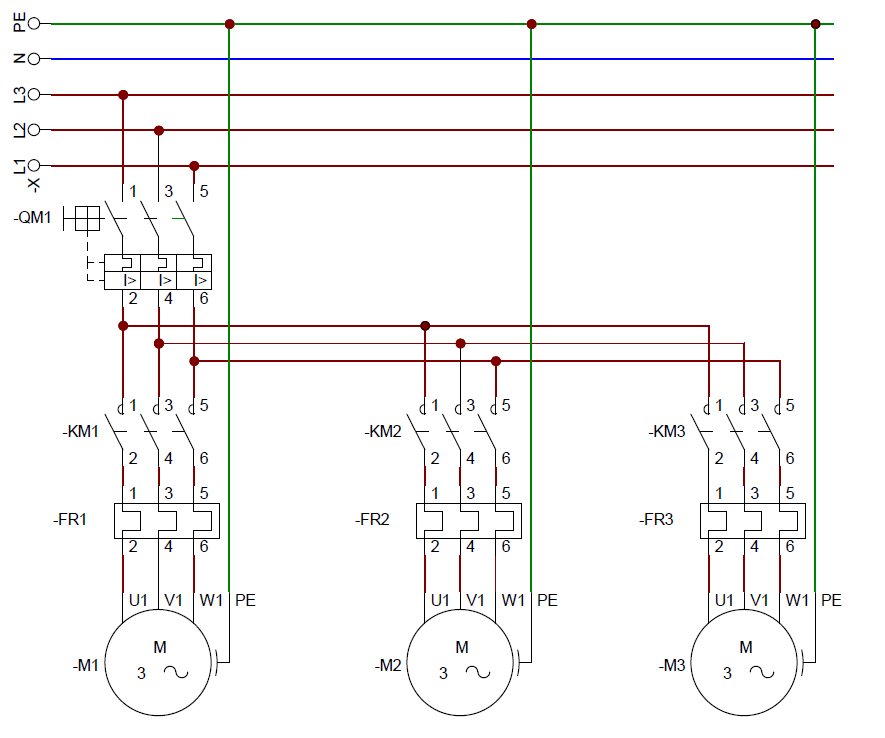
\includegraphics[width=\linewidth, height=10cm]{images/powerCircuit.png}
\end{figure}

\newpage
\subsection{Control circuit}
\begin{figure}[!ht]
    \centering
    \caption{Insert caption}\label{fig:controlCircuit}
    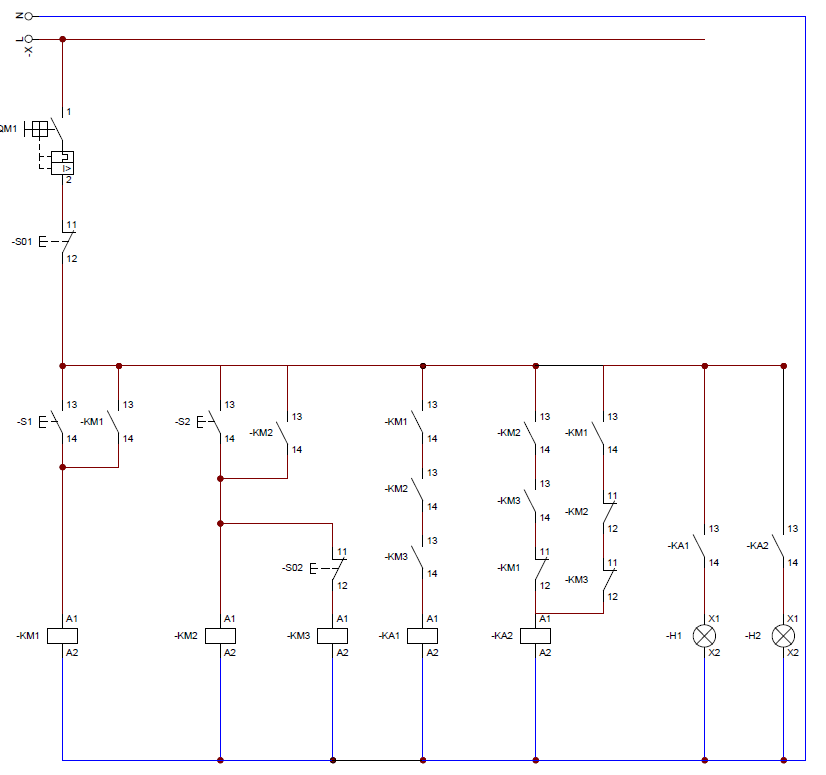
\includegraphics[width=\linewidth, height=15cm]{images/controlCircuit.png}
\end{figure}

% \bibliographystyle{splncs04}
% \bibliography{mybibliography}
\end{document}